\documentclass{llncs}
\pagestyle{plain}

%\usepackage[latin9]{inputenc}
%\usepackage[T1]{fontenc}
\usepackage{float}
\usepackage{wrapfig}
\usepackage{amsmath}
\usepackage{amssymb}
\usepackage{graphicx}
\usepackage{subcaption}
\captionsetup{compatibility=false}
% \usepackage{esint}
\usepackage{array}
\usepackage{epstopdf}
\usepackage{placeins}
\usepackage{url}
\usepackage{tikz}
\usepackage{calc}
\usepackage[linesnumbered,ruled,vlined]{algorithm2e}
\usetikzlibrary{positioning, arrows.meta,calc}
%%%%%%%%%%%%%%%%%%%%%%%%%%%%%%%
%%%%%%%%%%%%%%%%%%%%%%%%%%%%%%%

\newcommand{\vx}{\boldsymbol{x}}
\newcommand{\vW}{\boldsymbol{W}}
\newcommand{\vz}{\boldsymbol{z}}
\newcommand{\vb}{\boldsymbol{b}}








%\usepackage{amsmath, amsthm, amssymb, amsfonts}
%\newtheorem{theorem}{Theorem}
%\newtheorem{lemma}{Lemma}
%\newtheorem{corollary}{Corollary}
%\theoremstyle{definition}
%\newtheorem{definition}{Definition}



\newcommand{\ReLU}{\mathrm{ReLU}}



\title{I Compensate, therefore I Am \\ (accurate for DNN verification)}
\date{}

\begin{document}

\maketitle

\begin{abstract}
  Deep Neural Networks (DNNs) verification is now a mature research field, with many methodologies and tools to verify formaly  that they are correct, with an annual competition to compare them, etc. Formally, the question is, given a DNN and a property to check, does the property hold over a set of inputs of the DNN. This allows e.g. to check local robustness around an input $I$, by checking that the i-th output neuron has the largest weight among all output neurons uniformly over a neighbourhood around $I$.
  In the most recent years, the focus has been on combining several of these efficient techniques (branch and bound, multi neuron encoding, MILP encoding, ...) to optimize speed/accuracy trade-offs. While some relatively large DNNs (tens of thousands of neurons) can be checked very efficiently with modern tools, some DNNs are still challenging to address with efficient algorithms, even small ReLU DNNs with hundreds of neurons, showing the need for new methodologies.

  In this paper, we analyze efficient algorithms to verify ReLU DNNs, based on abstractions (DeepPoly, Linear Programing, PRIMA, different version of Crown), and uncover the main reason for the loss of accuracy, namely {\em compensations}. Intuitively, a compensation happens when there are 2 paths between the same pair of neurons, one path with positive and one path with negative (product of) weights, which therefore (partly) compensate each other. It is however hard to compute exactly by how much is the compensation due to the ReLU activation functions. Based on this finding, we propose a novel methodology to obtain interesting trade-offs in terms of speed/accuracy, using many queries with few 'open' ReLU nodes (for which both linear modes are considered), rather than the usual few queries with potentially many 'open' ReLU nodes. These promising results open up many different applications of the concept of compensating paths in the field of verification of DNNs.
\end{abstract}


\section{Introduction}

In the past 15 years, Deep Learning has revolutionized many tasks which were thought to be very hard to be handled by computers. This revolution however poses new challenges, as its automatically obtained product, namely Deep Neural Networks (DNNs), does not come with guidelines or rationale: it has tens of thousands of parameters (even for shallow networks with hundreds of neurons), it is very hard to understand, it is brittle to small perturbations \cite{szegedy}\dots

In this context, application of DNNs in safety critical applications is cautiously envisioned. For that to happen at a large scale, hard guarantees should be provided, so that to avoid dramatic consequences. It is the reason for the development of (hard) verification tools since 2016, with now many tools with different trade-offs from exact computation but slow (e.g. Marabou \cite{katz2019marabou}/Reluplex\cite{Reluplex}), up to very efficient but also incomplete (e.g. ERAN-DeepPoly \cite{deeppoly}). To benchmark these tools, a competition has been run since 2019, namely VNNcomp. The current overall better performing verifier is $\alpha$-$\beta$-Crown \cite{crown}, a fairly sophisticatedly engineered tool based mainly on "branch and bound" (BaB), and which can scale all the way from complete on smaller DNNs \cite{xu2020fast} up to very efficient on larger DNNs, constantly upgraded, e.g. \cite{cutting}.

While the verification engines are generic, the benchmarks usually focus on local robustness, i.e. given a Network, an image and a small neighbourhood around this image, 
is it the case that all the images in the neighbourhood are classified in the same way.
While some quite large DNNs (e.g. ResNet with tens of thousands of neurons) can be verified very efficiently (tens of seconds per input) \cite{crown}, with all inputs either certified robust or an attack on robustness is found; some smaller DNNs (with hundreds of neurons, only using the simpler ReLU activation function) cannot be analysed fully, with $12-20\%$ of inputs where neither of the decisions can be reached \cite{crown} and Table \ref{tab:example}. The main difference between these DNNs with very different behaviours lies in that the DNNs which are trained to be robust are much easier to verify, while the DNNs trained in a "natural" way are much harder to verify.


In this paper, we focus on DNNs trained in a "natural", 
%uncovering what makes the DNNs trained in a natural way so hard to verify (
because for "easier" DNNs, adequate methods already exist. 
To do so, we analyse the abstraction mechanisms at the heart of several efficient algorithms, namely Eran-DeepPoly \cite{deeppoly}, the Linear Programming approximation \cite{MILP}, PRIMA \cite{prima}, and different versions of ($\alpha$)($\beta$)-CROWN \cite{crown}. All these algorithms compute lower or/and upper bounds for the values of neurons (abstraction on values) for inputs in the considered input region, and conclude based on such bounds. For instance, if for all image $I'$ in the neighbourhood of image $I$, we have $weight_{I'}(n'-n) < 0$ for $n$ the output neuron corresponding to the expected class, then we know that the DNN is robust in the neighbourhood of image $I$. We restrict the formal study to DNNs using only the standard ReLU activation function, although nothing specific prevents the results to be extended to more general architectures. We uncover that {\em compensations} 
(see next paragraph) is the phenomenon creating inaccuracies. We verified experimentally that DNNs trained in a natural way have much more heavy compensating pairs than DNNs trained in a robust way.

Formally, a compensating pair is a pair of paths $(\pi,\pi')$ between a pair of neurons $(a,b)$, such that we have $w < 0 < w'$, for $w,w'$ the products of weight seen along $\pi$ and $\pi'$. Ignoring the (ReLU) activation functions, the weight of $b$ is loaded with $w \cdot weight(a)$ by $\pi$, while it is loaded with $w' \cdot weight(a)$ by $\pi'$. That is, it is loaded by $(w+w') weight(a)$. As $w,w'$ have opposite sign, they will compensate (partly) each other. The compensation is only partial due to the ReLU activation seen along the way of $\pi$ which can "clip" a part of $w \cdot weight(a)$, and similarly for $\pi'$. However, it is very hard to evaluate by how much without explicitly considering both phases of the ReLUs, which all the efficient tools try to avoid because it is very expansive (could be exponential in the number of such ReLU nodes opened).

Our first main contribution is to formally show, in Theorem \ref{th1}, that compensation is the sole reason for the inaccuracies as (most) efficient algorithms will compute exact bounds for all neurons if there is no compensating pair of paths at all.
While this theorem is theoretically interesting, it is not usable in practice as (almost) all networks have some compensating pairs. However, this notion of compensating pairs opens a first interesting idea concerning an exact abstraction of the network using a Mixed Integer Linear Program \cite{MILP}, where the weight of each neuron is a linear variable, and ReLU node may be associated with binary variables (exact encoding) or linear variables (overapproximation). While LP tools can scale to thousands of linear variables, MILP encoding can only be solved for a limited number of binary variables. This suggests that a simpler encoding could be used for those ReLUs that are not on compensating pairs, as their precise outcome may not be necessary.

Our second main contribution is to show formally in Theorem \ref{th2}, that 
encoding all ReLU nodes on a pair of compensating paths with a binary variable,
and using linear relaxation for the other ReLU nodes, will lead to exact bounds for (most) of the algorithms considered. This theorem allows to restrict the number of integer variables, and thus to obtain encodings that are faster to solve. Practically, however, (almost) all ReLU nodes are on some compensating path, and using this exact restricted MILP encoding will be too time consuming.

Our third main contribution is more practical, proposing Algorithm \ref{algo1} based on this knowledge that compensating pair of paths are the reason for inaccuracy. The idea is thus to use this information to rank the ReLU nodes in terms of importance, and only keep the most important ones as binary variables, and use linear relaxation for the least important ones.
%More precisely, the algorithm will, as DeepPoly, consider layers one by one and neurons $b$ %on this layer one by one, selecting the heaviest pairs of compensating paths ending in $b$
%and associating these nodes with a binary variable. Then an MILP tool such as Gurobi is used %to compute the lower and upper bound for node $b$. 
Overall, the worst case complexity of algorithm \ref{algo1} is lower than $O(N 2^K LP(N))$, where $N$ is the number of nodes of the DNN, $K$ the number of ReLU nodes selected as binary variable, and $LP(N)$ is the (polynomial time) complexity of solving a linear program representing a DNN with $N$ nodes. This complexity is an upper bound, as e.g. Gurobi is fairly efficient and never need to consider all of the $2^K$ ReLU configurations to compute the bounds. Keeping $K$ reasonably low thus provides an efficient algorithm. 
By design, it will never run into a complexity wall (unlike the full MILP encoding), although it can take a while on large networks because of the linear factor $N$ in the number of nodes. An additional interesting point is that it is extremely easy to parallelize, as all the nodes in the same layer can be run in parallel. We verify experimentally that the algorithm offers interesting trade-offs, by testing on local robustness for DNNs trained "naturally" (and thus difficult to verify).

This paper does not focus on producing the most efficient tool, and we did not spend engineering efforts to optimize it. The focus is instead on the novel notion of compensation, the associated methodology and its evaluation. For instance, our implementation is fully in Python, with uncompetitive runtime for our DeepPoly implementation ($\approx 100$ slower than in CROWN). Still, evaluation of the methodology versus even the most efficient tools reveals a lot of potential for the notion of compensation, opening up several opportunities for applying it in different contexts of DNN verification (see Section \ref{Discussion}). 

\smallskip

\noindent {\bf Comparison with related work:} Here, we will compare with several (but not all) main verification tools for DNNs, to better explain our methodology and how it differs with the existing SOTA. Compared with the exact encoding of a DNN using MILP \cite{MILP}, our algorithm can be seen as a way to help the MILP tool by telling it to not spend time to branch on ReLU nodes which have low impact on the particular node we are treating, at the cost of a small inaccuracy. If the ReLU nodes to abstract are chosen accurately, the result should be more accurate than early stopping the MILP algorithm using all the nodes.

Compared with the linear relaxation of the MILP encoding \cite{MILP}, our algorithm is strictly more accurate by design, but it will also be slower.

Compared with ERAN-Deeppoly \cite{deeppoly}, which compute bounds on the value in a very efficient way, we prove that the LP encoding is strictly more accurate, which as far as we know is another novel result. To be more precise, DeepPoly
abstract the weight of every node using two functions, one upper function and one lower function. While the upper function is fixed, there are 2 choices for the lower bound.
We prove in Proposition  \ref{LP} that the LP relaxation corresponds exactly to the intersection of both choices. It is thus more accurate than DeepPoly, but also not as efficient. Therefore, our algorithm will also be (much) more accurate than DeepPoly, but also not as efficient.

Concerning PRIMA \cite{prima}, the idea is to keep explicitly dependencies between neurons, computing bounds layer by layer (as we do). This allows to keep very efficiently dependencies from potentially many layers beforehand. We take care of dependencies between neurons in a different way, as compensation is the reason why there are dependencies between neurons. 
Our method is more accurate locally, but we will tend to lose precision for dependencies created many layers ago. Experimental results tend to show that most of the dependencies are local, in the few last layers (because ReLU nodes will likely clip those that happened many layers ago). Also, the dependencies between nodes limit the parallelism, unlike in our method, which explains why we obtain both faster and more accurate results than PRIMA.

For comparison, $\alpha$-$\beta$ CROWN \cite{crown} (and other Branch and Bound algorithms, such as BaB \cite{BaB}) will run few instances of branch and bound (one per output neuron), in worst case considering all the possible ReLU configurations (although the branch and bound algorithm avoids most of the possibilities). On simple networks, such as those trained robust, this is particularly efficient because branch and bound can find very efficiently the bounds focusing on the actual question, considering the important branches, while our algorithm will be less efficient as it has to consider each node one by one from the start. However, branch and bound faces a complexity wall when the network is hard to verify, such as the DNNs trained naturally, as there are too many branches to consider.

On such complex DNNs, PRIMA and $\alpha$-$\beta$ CROWN resort to a "refined" path, where the bounds {\em on the first few layers} are refined \cite{MILP2} using an exact MILP encoding. In our algorithm, we do not use an exact encoding but a partial one with the most important ReLU nodes obtained by considering the compensation strength. As it is more efficient, this can be pushed to all layers. This would be infeasible without the selection based on the compensation. The refined version of $\alpha$-$\beta$ CROWN is particularly accurate on small DNNs. As the depth grows, the more work is left to BaB and our algorithm is more accurate, lowering the gap of verified images to the upper bound \cite{attack} down from 
$20\%$ to $16.2\%$ and from $17.6\%$ to $12\%$ (depth 8, Table \ref{tab:example}). On larger naturally learnt DNNs (3000 neurons), BaB only verifies $18.5\%$ more images than DeepPoly (PRIMA only $6.5\%$), while our algorithm verifies $39\%$ more images than DeepPoly (Table \ref{tab:example3}).

Finally, algorithms abstracting the network (e.g. Reluplex / Marabou \cite{Reluplex,katz2019marabou}) are very different from algorithms abstracting the values (PRIMA, ($\alpha$)($\beta$)-CROWN)\cite{prima,crown}$\ldots$ These algorithms have been developed to be complete, so they are much slower but also more accurate than what we propose.



\section{Background}

In this paper, we will use lower case latin $a$ for scalars, bold for vectors $\boldsymbol{z}$, 
capitalized bold for matrices $\boldsymbol{W}$, similar to notations in \cite{prima,crown}.
To simplify the notations, we restrict the presentation to feed-forward, 
fully connected ReLU Deep Neural Networks (DNN for short), where the ReLU function is $ReLU : \mathbb{R} \rightarrow \mathbb{R}$ with
$ReLU(x)=x$ for $x \geq 0$ and $f(x)=0$ for $x \leq 0$, which we extend componentwise on vectors.

%In this paper, we will not use tensors with a dimension higher than matrices: those will be flattened.

%\subsection{Neural Network and Verification}


% testtesttesttest
An $\ell$-layer DNN is provided by $\ell$ weight matrices 
$\boldsymbol{W}^i \in \mathbb{R}^{d_i\times d_{i-1}}$
and $\ell$ bias vectors $\boldsymbol{b}^i \in \mathbb{R}^{d_i}$, for $i=1, \ldots, \ell$.
We call $d_i$ the number of neurons of hidden layer $i \in \{1, \ldots, \ell-1\}$,
$d_0$ the input dimension, and $d_\ell$ the output dimension.

Given an input vector $\boldsymbol{z}^0 \in \mathbb{R}^{d_0}$, 
denoting $\hat{\boldsymbol{z}}^{0}={\boldsymbol{z}}^0$, we define inductively the weight vector $\boldsymbol{z}^i$ at layer $1 \leq i \leq \ell$ with
\begin{align*}
	{\boldsymbol{z}}^{i} &= \boldsymbol{W}^i\cdot \hat{\boldsymbol{z}}^{(i-1)}+ \boldsymbol{b}^i\\
	\hat{\boldsymbol{z}}^{i} &= ReLU({\boldsymbol{z}}^i).
\end{align*} 

The vector $\hat{\boldsymbol{z}}$ is called post-activation values, 
$\boldsymbol{z}$ is called pre-activation values, 
and $\boldsymbol{z}^{i}_j$ is used to call the $j$-th neuron in the $i$-th layer. 
For $\boldsymbol{x}=\vz^0$ the vector of input, we denote by $f(\boldsymbol{x})=\vz^\ell$ the output. Finally, neurons are also called \emph{nodes}, and when we refer to a specific neuron, we use $a,b,c,d$ to denote them, and $W_{a,b} \in \mathbb{R}$ to denote the weight from neuron $a$ to $b$. Similarly, for input $\boldsymbol{x}$, we denote by $weight_{\boldsymbol{x}}(a)$ the weight of neuron $a$ when the the input is $\boldsymbol{x}$. A path $\pi$ will be a sequence 
$\pi=(a_i)_{k \leq  i \leq k'}$ of neurons in consecutive layers, and the weight $w(\pi)=W_{a_k,a_{k+1}} \times \cdots \times  W_{a_{k'-1},a_{k'}}$.





\iffalse
and the $i$-th hidden layer is a vector in $\mathbb{R}^{d_i}$, 
and the output layer is a vector in $\mathbb{R}^{d'}$ or a scale. 
The weights, bias and activation functions decide propagate the from previous to the next layer. In formula, from layer $l_{i-1}$ to layer $l_{i}$, the weight 
$\boldsymbol{W}^i$ is matrix of $d_i\times d_{i-1}$, 
the bias is a vector $\boldsymbol{b}^i$ in $\mathbb{R}^{d_i}$, and the activation function 
is $\sigma$, then  if the $i-1$-th layer is $\hat{\boldsymbol{z}}^{(i-1)}$, 
then the value of $i$-th layer is computed by: 
\begin{align*}
	{\boldsymbol{z}}^{i} &= \boldsymbol{W}^i\cdot \hat{\boldsymbol{z}}^{(i-1)}+ \boldsymbol{b}^i\\
	\hat{\boldsymbol{z}}^{i}(n) &= \sigma({\boldsymbol{z}}^i(n)).
\end{align*} The vector $\hat{\boldsymbol{z}}$ is called post-activation values, and $\boldsymbol{z}$ is called pre-activation values, and $\boldsymbol{z}^{(i)}_j$ is used to call the $j$-th neuron in the $i$-th layer. In our style, we also call neurons \emph{nodes} and use $a,b,c,d$ to denote them. We use $W_{ab}$ to denote the weight from neuron $b$ to $a$. We use $\boldsymbol{x}$ to denote the vector of input and  $f(\boldsymbol{x})$ to denote the output.
\fi

\medskip

Concerning the verification problem, we focus for simplicity on the usual local robustness question. Local robustness asks to determine whether the output of a neural network will be affected under small perturbations to the input. 
Formally, for an input $\vx$ perturbed by $\varepsilon >0$ under distance $d$, then the DNN is locally $\varepsilon$-robust in $\vx$ whenever:
\begin{align*}
	\forall \boldsymbol{x'} \text{ s.t. } d(x,x')\leq \varepsilon, \text{ we have }  
	argmax_i (f(\boldsymbol{x'})[i]) = argmax_i(f(\boldsymbol{x})[i])
\end{align*} 

\iffalse
In some cases, the output is a vector but the aim to get the label of dimension with the minimal value. In this case, the problem can be written as:\begin{align*}
\forall \boldsymbol{x} \in\mathcal{D} \  \min f(\boldsymbol{x}) = \min f(\boldsymbol{x}_0)
\end{align*}

If so, the question of verification can turn to the following optimization question: \begin{align*}
	\min f(\boldsymbol{x}) \ s.t. {\boldsymbol{z}}^{i} &= \boldsymbol{W}^i\cdot \hat{\boldsymbol{z}}^{(i-1)}+ b^i\\
	\hat{\boldsymbol{z}}^{i}(n) &= \sigma({\boldsymbol{z}}^i(n)), \boldsymbol{x}\in\mathcal{D}.
\end{align*}

In this paper, we only consider $\ReLU$ function as the activation function: $\sigma(a)=\ReLU(a)=\max(0,a)$. 

In this paper, we consider $L^{\infty}$ norm the max value of distance of each dimension, that is $d(\boldsymbol{x},\boldsymbol{x}_0)=\max |\boldsymbol{x}(n)-\boldsymbol{x}_0(n)|$. 
\fi


\section{Value Abstraction for DNN verification}


\begin{figure}[t!]
	\centering
		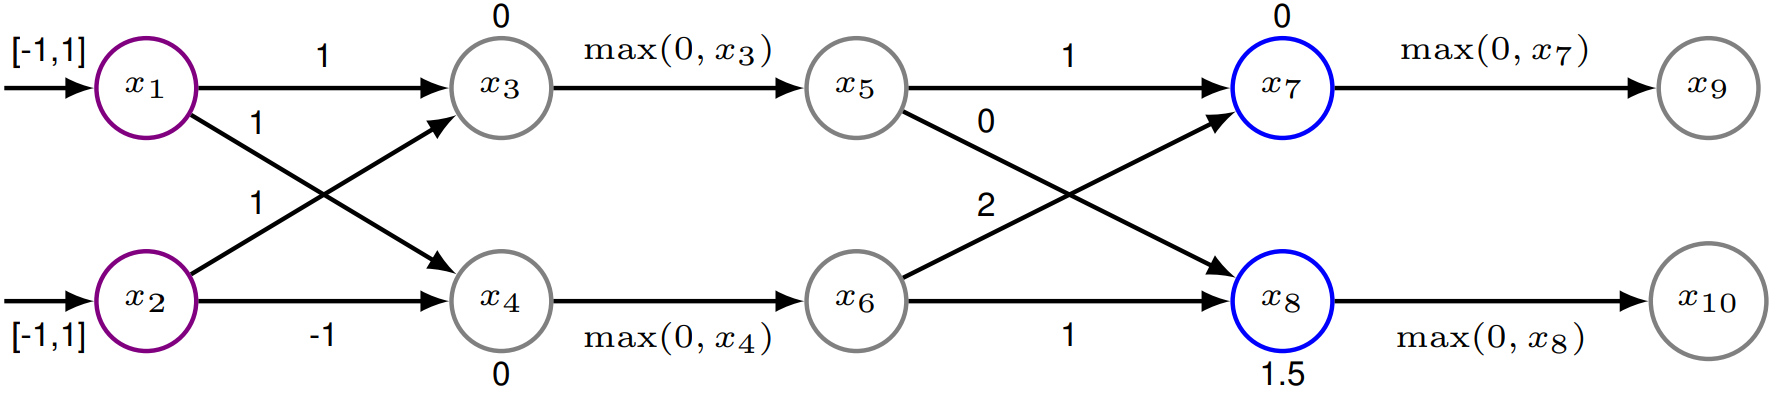
\includegraphics[scale=0.4]{example.png}
	\caption{A DNN example from \cite{kneuron}}
	\label{fig1}
	\end{figure}
	

An efficient and prolific line of work concerning DNN verification has been to develop value abstraction of the network. The idea is to compute upper and lower bounds on the values of (some) neurons in the DNN when the inputs are in a given neighbourhood, in order to conclude on the robustness without needing to compute the values exactly for all inputs.

Consider the simpler abstraction, called the box abstraction \cite{deeppoly}: from the bounds in the input, one compute by the linear step the bound on the next layer, apply the ReLU function, and so on.
For instance, on the DNN example of Fig \ref{fig1}, 


\subsection{MILP formation of $\ReLU$ functions}

In literature, many methods have been used to approximate $\ReLU$ functions. One of them is MILP (or MIP, Mixed Integer Linear Programming).

For a activation $x=\ReLU(y)$, if we already know $y's$ rough upper and lower bounds $u,l$, then if $u>0$ and $l<0$, we call $y$ is unstable; otherwise, $y$ is stable. In practice, stable node is easier because $\ReLU$ function becomes a linear function on this node. The key problem is to deal with unstable nodes.

In literature, if $x=\ReLU(y)$, and $y$ is unstable, then this function can be formulated in MILP with one integer variable $a$ valued in ${0,1}$ (i.e., a binary variable) by:

\vspace*{-4ex}

\begin{align*}
	&x \geq 0, \ 
	x \geq y-l\cdot (1-a)\\
	&x \leq y,\ 
	x \leq u\cdot a
\end{align*} 

MILP becomes one of standard methods to compute the lower bounds and upper bounds of neurons in a pure $\ReLU$ activation network. Combining with the discussion from previous subsection, the verification problem is equivalent to an MILP optimization problem.


However, the cost of optimization of an MILP model is very expensive, especially when the number of binaries increases: solving MILPs are NP-hard, and often needs exponential time to solve it. A typical relaxation is to change the binary variable $a$ to a continue variable, then it will be equivalent to the standard triangle LP model for $\ReLU$ function.

Our strategy is to restrict the number of binary variables, and this will definitely lose accuracy of results.  The key problem is how to use fewer binary variables to get more accuracy. That is, to choose which node to be binary, and which not.

\begin{definition}
	1. For a full-connected DNN with $\ReLU$ activation, to compute the upper or lower bound of a node (in a hidden layer or output layer), its MILP model is formulated as follows: 
	
	(1) For every node in the input layer $a$, set a $z_a$ variable with the same input interval: $l_a\leq z_a\leq u_a$
	
	(2) For each hidden layer $l^i$, set two variables , $z_c,\hat{z}_c$ for each node $c$ in this layer for pre-activation and post-activation. 
	
	The constraints for pre-activation $z_a$ is the natural linear equation by the network. 	$$z_c=\sum_{d\in l^{i-1}} W^i_{cd} z_d+b^i_c.$$
	
	
	The constraints for $\hat{z}_a$ is defined by the standard MILP formulation mentioned above with known upper bound and lower bound as parameters.
	
	\vspace*{1ex}
	
	Since we only consider such MILP models, so when we say an MILP model, it is for a full-connected DNN with $\ReLU$ activation. 
	
	2. In an MILP model, we say a $\ReLU$ node is open, if the binary variable corresponds to this function is still an binary variable; otherwise, it is relaxed as a continue variable. 
\end{definition}

We aim is to find an algorithm, to decide which nodes should be opened such that we can have more accuracy.

\section{Compensate, Diamond and Node Chosen}

In this section, we will explore the key factor for the loss of accuracy in our LP/MILP models: \emph{compensating pair}. And we will develop a process of open node chosen by the principle of \emph{Compensating Pairs}. 



\subsection{Compensating pair}

The basic mode of compensating pair is as follows:

\vspace*{2ex}

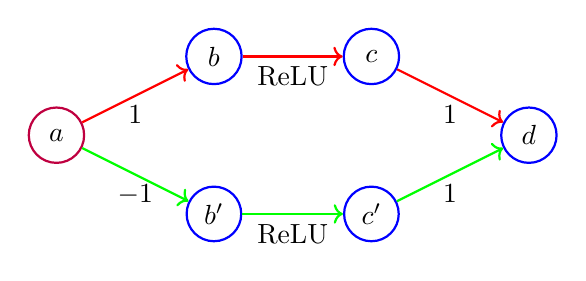
\begin{tikzpicture}
	\node[circle, draw= purple, thick, minimum width = 20,
	minimum height = 20] (input1) {$a$};

	
	% Hidden layers
	\node[circle, draw= blue, thick, minimum width = 20,
	minimum height = 20] (hidden1) at ($(input1) + (2,1)$) {$b$};
	\node[circle, draw= blue, thick] (hidden2) at ($(input1) + (2,-1)$) {$b'$};
	
	\node[circle, draw= blue, thick, minimum width = 20,
	minimum height = 20] (hidden3) at ($(input1) + (4,1)$){$c$};
	\node[circle, draw= blue, thick] (hidden4) at ($(input1) + (4,-1)$) {$c'$};
	
	% Output layer
	\node[circle, draw= blue, thick, minimum width = 20,
	minimum height = 20] (output) at ($(input1) + (6,0)$){$d$};
	
	% Connections
	\draw[->,thick,draw= red] (input1) -- (hidden1) node[midway, below] {$1$};
	\draw[->,thick,draw= green] (input1) -- (hidden2)node[midway, below] {$-1$};
	
	\draw[->,thick,draw= red] (hidden1) -- (hidden3) node[midway, below] {$\ReLU$};
	\draw[->,thick,draw= green] (hidden2) -- (hidden4) node[midway, below] {$\ReLU$};
	
	\draw[->,thick,draw= red] (hidden3) -- (output)node[midway, below] {$1$};
	\draw[->,thick,draw= green] (hidden4) -- (output)node[midway, below] {$1$};
\end{tikzpicture}

\vspace*{2ex}

In this figure, $a$ is the input neuron; $bc,b'c'$ are nodes in the hidden layer, ($b,b'$ are pre-activation and $c,c'$ are post activation); and $d$ is the unique output neuron. The numbers next to the arrows are the weights. So, $W_{ba}=1$ and $W_{b'a}=-1$, $W_{dc}=W_{dc'}=1$. The pair of these two paths, $a$ to $bc$ to $d$, and $a$ to $b'c'$ to $d$, is a so called \emph{Compensating Pair}. Because its shape looks like a diamond, it is also called a Diamond. The characteristic is that, the products of all weights in the paths, have two different signs: along $bc$, the product is (strictly) positive, while along $b'c'$, the product is (strictly) negative. 

The existence of compensating pairs is key reason why simple approximation like LP or Interval Arithmetic cannot get the exact upper and lower bounds. If both pairs are negative or positive, LP or even Interval Arithmetic will get the exact values of lower and upper bounds.


To explain why, suppose we have another input node $a'$, such that both $a$ and $a'$ has an input interval $[0,1]$, but the weight from $a'$ to $b$ or $b'$ are both $1$. Then both $b$ will have an interval $[0,2]$ and $b'$ will have an interval $[-1,1]$. More importantly, in LP formulation, $c$ will be $b$ but $c'$ will be $0.5(b')+0.5$. The upper bound of $d$ will be $c+c'$, and hence $b+0.5(b')+0.5$, and hence $a+a'+0.5a'-0.5a'+0.5=0.5a+1.5a'+0.5$. And this will leads to a upper bound $2.5$ but this is not exact.

\vspace*{2ex}
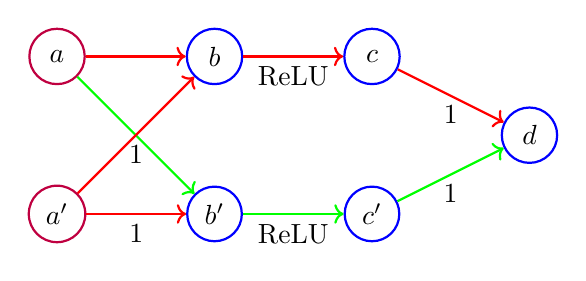
\begin{tikzpicture}
	\node[circle, draw= purple, thick, minimum width = 20,
	minimum height = 20] (input1) {$a$};
	
	\node[circle, draw= purple, thick, minimum width = 20,
	minimum height = 20] (input2) at ($(input1) + (0,-2)$) {$a'$};
	
	
	% Hidden layers
	\node[circle, draw= blue, thick, minimum width = 20,
	minimum height = 20] (hidden1) at ($(input1) + (2,0)$) {$b$};
	\node[circle, draw= blue, thick] (hidden2) at ($(input1) + (2,-2)$) {$b'$};
	
	\node[circle, draw= blue, thick, minimum width = 20,
	minimum height = 20] (hidden3) at ($(input1) + (4,0)$){$c$};
	\node[circle, draw= blue, thick] (hidden4) at ($(input1) + (4,-2)$) {$c'$};
	
	% Output layer
	\node[circle, draw= blue, thick, minimum width = 20,
	minimum height = 20] (output) at ($(input1) + (6,-1)$){$d$};
	
	% Connections
	\draw[->,thick,draw= red] (input1) -- (hidden1);
	\draw[->,thick,draw= green] (input1) -- (hidden2);
	
	\draw[->,thick,draw= red] (input2) -- (hidden1) node[midway, below] {$1$};
	\draw[->,thick,draw= red] (input2) -- (hidden2)node[midway, below] {$1$};
	
	\draw[->,thick,draw= red] (hidden1) -- (hidden3) node[midway, below] {$\ReLU$};
	\draw[->,thick,draw= green] (hidden2) -- (hidden4) node[midway, below] {$\ReLU$};
	
	\draw[->,thick,draw= red] (hidden3) -- (output)node[midway, below] {$1$};
	\draw[->,thick,draw= green] (hidden4) -- (output)node[midway, below] {$1$};
\end{tikzpicture}
\vspace*{2ex}

The general formal definition of compensating pair is as follows:

\begin{definition} In a full-connected network with $\ReLU$ as activation function:
	
	1. A path is a sequence of nodes $\langle a,b,c,d,e,\cdots\rangle$ of nodes that goes consecutively through each layer. We call the first node source node and the last node target node.  
	
	2. The \emph{Value} of a path is the product of of weights along the path (with sign): for a path $\langle a,b,c,d,e,\cdots\rangle$, its values is $$V = W_{ab}\cdot W_{bc}\cdot W_{cd}\cdot W_{ed}\cdot \cdots$$
	
	3. A \emph{Compensating Pair} is a pair of paths with the same source node and target node, such that the two paths have no common node, and the values of two paths have opposite signs (one is strictly positive and another is strictly negative).
	
	We also use \emph{Diamond} to call a compensating pair in the network.
\end{definition}


The following theorem shows the role of compensating pairs in the computation:

\begin{theorem}[No Diamond Theorem, part 1]
	For a full-connected network with $\ReLU$ as the unique activation function, if there is no Diamond, then for any method/approximation that at least as accurate as Interval Arithmetic, it can get the exact upper and lower bounds of all output nodes and all hidden nodes.
\end{theorem}

Of course, in practice, it is very unlike to have a network without any Diamond. Therefore, the second theorem is more important in practice.

\begin{theorem}[No Diamond Theorem, part 2]
	For a full-connected network with $\ReLU$ as the unique activation function. If we open all nodes that occurs in a compensating pair path, then the we can get the exactly bounds.
\end{theorem}

The proofs of above theorems are in the Appendix.

\subsection{Paths and Open Nodes Chosen}

In this subsection, we will introduce the method to choose open nodes for MILP model based on compensating pairs.

Based on No Diamond Theorem, for a target node, in its MILP model, if we open all nodes in compensating pairs, then we can get the exact values of upper and lower bound of the target node. However, in practice, this is still too expensive because we will still need to open too many nodes. So we can only choose a limited number of compensating pairs and nodes. This is by setting a parameter $O$ such that the process only choose at most $O$ many nodes to open. Therefore, in this subsection, we will introduce the process of open node chosen: given a target node, choose up to $O$ many nodes to open.


Basically, we do the process of open nodes chosen for one target node each time, that is, receive one target node (and other data) as input each time. But in principle, we can develop a method receive more than one nodes as input. But in our experiences, this does not work well.  

This process is not the unique method but the most natural way to choose open nodes. We introduce it in three steps from the simplest case to more complex case.

\subsubsection*{Value of a pair}


For a compensating pair, if $V_1,V_2$ are the values of two paths, then the value of this compensating pair is defined by: $V=\min(|V_1|,|V_2|)$.


\subsection*{Case: Source node fixed}

The simplest case is when we only consider compensating pairs with a fixed source node. 

In this case, the process is very simple: enumerate all compensating pairs, and then sort them by their values. Finally, from the first to the last compensating pair, pick all unstable nodes in its two paths except the target and source nodes into the list of open nodes, until $O$ many open nodes. 

%\subsubsection*{Sort all paths by values}
%
%The first step is to sort all paths by their values and divide paths into two groups, a group of paths with positive values and a group of paths with negative values.
%
%Since we have set a bound $O$ for open nodes, we will store  a fixed number of path for each group.
%
%\subsubsection*{Sort pairs by values}
%
%The second step is to sort all pairs by their values. Enumerate paths from the positive group and the negative group one by one and put the pairs obtained into a new list of pairs. Then sort all pair by their values from largest to the smallest: recall that the value of a pair $\langle P_1,P_2\rangle$ is $\min(|V_1|,|V_2|)$.
%
%\subsubsection*{Choosing nodes}
%
%The third step is to choose nodes from the list of pairs. According to the sorted list of pairs, enumerate pair one by one; for each pair, pick the nodes unstable in the two paths except the source and target node into the open node list. Repeat this process until $O$ nodes chosen or reach the end of the list.
%
%\subsubsection*{Pseudocode}
%
%The following needs a chart of pseudo-code
%
%\vspace*{1ex}
%
%1. Enumerate all path from the fixed source node to the target node. 
%
%2. For each path, compute its weight, that is the products of all $W_{aa'}$ along the path.
%
%3. Divide all paths into two group: positive paths and negative paths.
%
%4. Pair positive paths and negative paths from those with larger absolute values to smaller. 
%
%5. For each pair, its value is the min of the weight positive paths and absolute negative values.
%
%6. From pairs with larger values to smaller, pick path one by one, and check all intermediate nodes (nodes except source and target) of each path, and if any of them is unstable ($u>0$ and $l<0$), then open this node. 
%
%7. Repeat 6 until choosing sufficiently many nodes.
%





\subsection*{Case: Source nodes in one layer}

The more general case is when the source node can be any node in a fixed layer. In this case, the process is very similar to previous case, except the value of a pair.

In this case, for a pair $P_1,P_2$ with values $V_1,V_2$ with the source node $a$, its value is $\min(|V_1|,|V_2|)\times \text{upper bound of } a$.

%\subsubsection*{Pseudocode}
%
%The following needs a chart of pseudo-code
%
%\vspace*{1ex}
%
%1. Enumerate all path from the fixed source node to the target node. 
%
%2. For each path, compute its weight, that is the products of all $W_{aa'}$ along the path.
%
%3. Divide all paths into two group: positive paths and negative paths.
%
%4. Pair positive paths and negative paths from those with larger absolute values to smaller. 
%
%5. For each pair, its value is the min of the weight positive paths and absolute negative values, times the upper bound (at least 0) of the source node.
%
%6. From pairs with larger values to smaller, pick path one by one, and check all intermediate nodes (nodes except source and target) of each path, and if any of them is unstable ($u>0$ and $l<0$), then open this node. 
%
%7. Repeat 6 until choosing sufficiently many nodes.







\subsection*{Case: Source nodes in different layers}

The general case is that when the location of source nodes can be in different layers. This case is much more complex, because the scale level of values of paths from different layers are very different: usually a weight will be very small since every layer has a large number of nodes, therefore values of longer paths are products of more small numbers, and is definitely much smaller. If we sort all compensating pairs from different layers directly, then a very long initial segment of this list will be occupied by compensating pairs with the shortest length. Therefore, we need use some scale factors when comparing values of compensating pairs of different length.

In our experiments, we only consider the paths of length 3 (the source node is 2 layers before) and length 4 (the source node is 3 layers before). We will dynamically adjust the values during the process of node chosen. In text, the process of node chosen for length 3 plus length 4 is as follows:

\vspace*{1ex}

1. Generate the two lists of pairs sorted by their values for source nodes in 2 layers before the target node and 3 layers before separately as in the previous case.

2. Enumerate pair from two lists one by one by their values and pick nodes as previous case. When comparing the values between pairs of length 4 and pairs of length 3, multiply the numbers of nodes in 1 layer before to the value of pair of length 4.

In formula, when the target node is in layer $L$, for a pair $P_3$ of length 3 with value $V_3$ and a pair $P_4$ of length 4 with value $V_4$, if we have chosen $N$ nodes in layer $L-1$. Then the adjusted values for $P_3$ and $P_4$ are: $$V_3, N\cdot V_4.$$ Then we pick the next pair by the adjust value in two lists.

3. Repeat 2 until choosing sufficiently many nodes.

\vspace*{1ex}

The pseudo-code is as follows ():

\begin{algorithm}
	\caption{Process for length 3 + length 4}
	\KwData{Sorted lists of length 3 + length 4}
	\KwResult{Open node list}
	
	Let $N = 0$ be the number of Chosen length 4 pair.
	
	\While{len(Open node) $<O$}{
		Pick the first element $P_3$ in the list of length 3\;
		
		Let $V_3$ be the value of $P_3$\;
		
		Pick the first element $P_4$ in the list of length 4\;
		
		Let $V_4$ be the value of $P_4$\;
		
		\If{$V_3 > V_4 \cdot N$}{
			Add nodes in $P_3$ into Open list\;
			Number of Chosen lentgh pair $N$ += 1\; 
		}
		\Else{
			Add nodes in $P_4$ into Open list\;
		}
	}
\end{algorithm}


\section{Verification Framework}



%Our experiments are carried by different version codes, and the global process has been changed. 

In this section, we will sketch the framework. 

\subsection{Structure}

\subsubsection*{Precomputation}

The open node chosen is the key part of the whole framework but costs a lot of time. So some computation (those do not rely on certain image and bounds) is moved to the precomputation part.

%The precomputation corresponds to the simplest case: source node fixed. We will compute and store a limited number of paths with highest (absolute) values before running any image. This does not rely on other parameters or results(bounds).
%
%Before build an MILP model and when choosing open nodes list,  the program will read the reference data combining with the data of bounds to continue the computation of open nodes. This will use much less time.



\subsubsection*{Process for one image} An image is the basic unit in whole process. The process of one image is simple: compute the concrete bounds of nodes layer by layer, use the bounds of previous layer to build MILP models of current layer. In one layer, nodes runs in parallel.

%Suppose we have reached a new layer $l_i$ and have upper and lower bounds of all nodes in previous layers. Then we will compute bounds of every node in $l_i$ in parallel using the data of bounds of previous nodes. The method is to build and optimize an MILP model.

%Some parameters may be changed during layers. Among all parameters, two groups are the most important: numbers of open nodes and local timeout parameters. Here, \emph{local} is opposite to \emph{global}. We have global timeout parameters for images and the whole running. Local timeout are used in one layer, one node, one model, or one loop in the optimization for a model.




%The open node chosen is the key part of the whole framework, and it will cost two much time without precomputation because we must do open node chosen for every node. 
%
%The precomputation corresponds to the simplest case: source node fixed. We will compute and store a limited number of paths with highest (absolute) values before running any image. This does not rely on other parameters or results(bounds).
%
%Before build an MILP model and when choosing open nodes list,  the program will read the reference data combining with the data of bounds to continue the computation of open nodes. This will use much less time.


\subsubsection*{Process for one node}

 The optimization of a model consists of loops. For each loop, the model will do optimization by a timeout and observe the result. If it gets improvement, then continue the loop until the optimize bounds or the longer timeout. Otherwise it will give up optimization and store the best bounds obtained so far.  



\subsubsection*{Global Process}

In the newest version, we do images by batches for 100 images each. For each batch, the running consists of three turns, very fast turn, fast turn and slow turn.

In the very fast turn, it will run DeepPoly for all images to get a preliminary bounds for all nodes and verify the easiest images. Images verified and images with false predication will be deleted from the image list.

Then sort all remain images by the size of uncertainty of DeepPoly from smaller to larger. The fast turn is to run the images from the smaller side to larger side until consecutive two images cannot be verified. All remain images and images tried but not verified will be put into the next list. And then run the list with parameters for slow turn.




\subsection{Parameters}

Parameters like open node parameter $O$ is important in the frame. Basically, all parameters will be reset after one image.

\subsubsection*{Global parameters}




\subsubsection*{Local parameters}

$O$ and timeout parameters for loops will change frequently during the loops of one node. These change will not reset until the end of one layer or one image.



\subsection{Other Setting}

In our experiments, we have not used PGD-attack to exclude some images. In principle, there is no obstacle to use PGD-attack.



\section{Experimental Evaluation}

The neural network certification benchmarks for fully connected networks were run on a 32 core
GHz Intel with 256 GB of main memory. We use Gurobi 9.52 for solving MILP and LP problems


We used MNIST image datasets for our experiments. MNIST contains grayscale images of size 28 × 28 pixels. For our evaluation, we chose the first
1000 images from the test set of each dataset.

Each data example is associated with an $L^\infty$ norm $\varepsilon$ and a target label
for verification.

\subsection{Experiments about Node Chosen}

The first group of experiments is to test the direct effect of node chosen by compensating pair, comparing to random chosen. We use the average of uncertainty of all nodes in a layer to measure the effect of node chosen: for a node $a$, its uncertainty $UN(a) = UB(a)-LB(a)$, and the average uncertainty of a layer $l$ is $$UN(l) = \dfrac{\sum_{a\in l}UN(a)}{|l|}.$$

The test neural network is MNIST fully-connected $6\times 100$, and the test image is the image 59 in the MNIST image dataset. 

\subsubsection*{Node chosen in second hidden layer}

The following table shows the average uncertainty of the second hidden layer when choosing different numbers of open nodes by random or by compensating pairs.

\begin{table}
	\centering
	\begin{tabular}{c|c|c}

	\text{Number of open nodes}  &  \text{Compensating} & \text{Random}  \\ \hline
	0  &  2.22 & 2.22  \\ \hline
	10  &  1.84 & 2.03  \\ \hline
	20  &  1.50 & 1.82  \\ \hline
	30  &  1.28 & 1.62  \\ \hline
	40  &  1.14 & 1.44  \\ \hline
	50  &  1.06 & 1.23  \\ \hline
\end{tabular}
\caption{}
\label{tab:example0}
\end{table}



\subsubsection*{Node chosen in the third hidden layer}

The following table shows the average uncertainty of the third hidden layer when choosing different numbers of open nodes, by random or by compensating pairs.


\begin{table}
	\centering
	\begin{tabular}{c|c|c}
	
	\text{Number of open nodes}  &  \text{Compensating} & \text{Random}  \\ \hline
	0  &  1.758 & 1.758  \\ \hline
	10  &  1.677 & 1.695  \\ \hline
	20  &  1.539 & 1.622  \\ \hline
	30  &  1.431 & 1.542  \\ \hline
	40  &  1.329 & 1.47  \\ \hline
	50  &  1.243 & 1.39  \\ \hline
\end{tabular}
\caption{}
\label{tab:example1}
\end{table}



\subsection{Experiments Results}






\subsection{Comparison to Incomplete Verifiers}

In Table 3, we compare against two representative incomplete
verifiers on 4 MLP networks for MNIST under the same
set of 1000 images. beta-Crown is the state-of-the-art verifier based on branch-and-bound. PRIMA is another strong and representative method based on multi-neuron linear relaxation.

\begin{table}
	\centering
	\begin{tabular}{c|c|cc|cc|cc|cc}
		
		\text{Network}  & $\varepsilon$&  \multicolumn{2}{@{}c@{}|}{\text{Comp(fast)}} & \multicolumn{2}{@{}c@{}|}{\text{PRIMA}} &  \multicolumn{2}{@{}c@{}|}{\text{Comp(slow)}} & \multicolumn{2}{@{}c@{}|}{\text{beta-Crown}}  \\ 
		
		&  & \textrm{Ver}.\% & \textrm{Time}(s) & \textrm{Ver}.\% & \textrm{Time}(s) &\textrm{Ver}.\% & \textrm{Time}(s) & \textrm{Ver}.\% & \textrm{Time}(s) \\ \hline
		
		\textrm{MLP}\ 5$\times$100\  &   0.026& 1.758 & time & 51 & 159 &    68.4 & 142 & 69.9 & 102 \\ \hline
		
		\textrm{MLP}\ 8$\times$100\  &   0.026& 52.7 & 92.3 & 42.8 & 301 &    65.8 & 364 & 62 & 103 \\ \hline
		
		\textrm{MLP}\ 5$\times$200\  &   0.015& 1.758 & time & 69 & 224 &    76.8 & 279 & 77.4 & 86 \\ \hline
		
		\textrm{MLP}\ 8$\times$200\  &   0.015& 68.1 & 297 & 62.4 & 395 &    79.1 & 535 & 73.5 & 95 \\ \hline
		
		\textrm{MLP}\ 6$\times$500\  &   0.035& 1.758 & time & 1.758 & time &    1.758 & time & 1.758 & time \\ \hline
	\end{tabular}
	\caption{The data of verified accuracy (\%) and average time (s) of 1000 images evaluated on the PRIMA and on the beta-Crown are in CITE.}
	\label{tab:example}
\end{table}

On all 4 networks, our fast version can exceed PRIMA both in accuracy and speed. On all 4 networks, our slow version can have a similar verified accuracy as beta-Crown.

% test

\section{Related Work}

\section{Conclusion}

\section*{Appendix: Proofs of No Diamond Theorem}


\bibliographystyle{plain}
\bibliography{references}


\end{document}


